\chapter{วิธีการทดลอง}
\label{chapter:experiment}

ในบทนี้เรากล่าวถึงวิธีการใหม่ของเราที่ได้ปรับปรุงและพัฒนาขึ้นมาโดยใช้ SWT เป็นส่วนหลักในของระบบใหม่ โดยมีจุดประสงค์เพื่อทำให้สามารถใช้งานร่วมกับภาพมังงะได้อย่างมีประสิทธิภาพ และดำเนินการทดลองเพื่อวัดประสิทธิภาพของวิธีการใหม่ของเราว่าสามารถทำงานได้ดีขึ้นหรือไม่อย่างไรเมื่อเปรียบเทียบกับวิธีการต้นฉบับ~\cite{5540041} และวิธีการอื่น ๆ ที่ถูกพัฒนามาก่อนหน้า

\section{วิธีการใหม่ที่ถูกปรับปรุงและพัฒนาเพิ่มเติม}

สำหรับวิธีการอย่างที่ได้กล่าวไปในบทที่~\ref{chapter:introduction} วิธีการใหม่ของเราได้ใช้ประโยชน์จาก SWT ร่วมกับความสามารถของ SVM โดยใช้ HOG เป็นลักษณะเด่น หรือ Feature อย่างไรก็ดีตามที่ได้กล่าวไปในบทที่~\ref{chapter:introduction} จุดประสงค์หลักของ SWT ที่ถูกนำเสนอไปในงานวิจัยก่อนหน้านั้นถูกออกแบบเพื่อการตรวจหาข้อความบนภาพถ่ายเป็นเป้าหมายหลัก ด้วยเหตุผลนี้ทำให้การทำงานร่วมกับภาพมังงะไม่สามารถทำงานได้ดีอย่างที่ควร ก่อให้เกิด False Positive จำนวนมาก ตามที่แสดงให้เห็นในภาพ~\ref{Fig:similar} ซึ่งจำนวน False Positive ที่มากนั้นแสดงถึงประสิทธิภาพที่ต่ำของระบบ สาเหตุหลักคือความแตกต่างเชิงเอกลักษณ์ของวัถตุในภาพจริงและภาพวาดมังงะ นอกจากนี้องค์ประกอบต่าง ๆ ในภาพวาดของมังงะนั้นยังมีความคล้ายคลึงกับลักษณะของตัวอักษรในภาพมากเกินไป เช่น เส้นของต้นหญ้า, เส้นผมของตัวละคน, และรายละเอียดบนพื้นหลัง อย่างที่แสดงในภาพ~\ref{Fig:similar:1} และภาพ~\ref{Fig:similar:3} ด้วยเหตุนี้วิธีการของเราจึงปรับปรุงขั้นตอนของระบบดังเดิม โดยเราได้ปรับปรังขั้นตอนการค้นหาวัตถุที่คล้ายคลึงอักษร, การจับกลุ่มอักษร, และเพิ่มขั้นตอนใหม่สำหรับการคัดแยกอักษรเพิ่มอีกหนึ่งขั้นตอน เพื่อให้สามารถใช้งานกับมังงะได้อย่างมีประสิทธิภาพและแม่นยำมากขึ้น

\begin{figure}[!h]
    \centering
    \subfigure[]{
        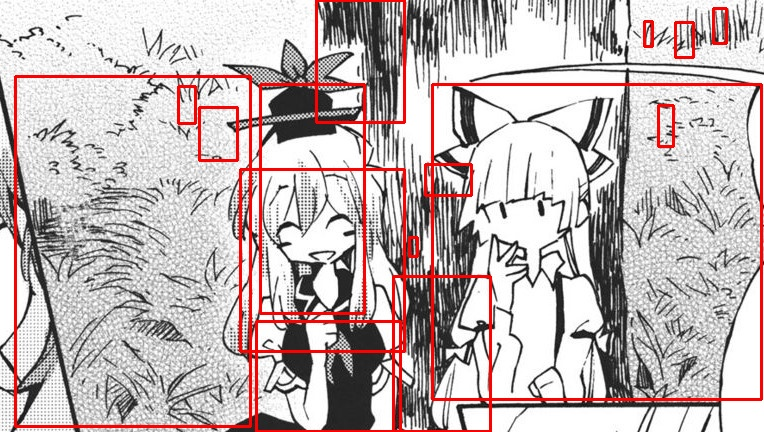
\includegraphics[width=0.7\columnwidth]{images/similar-obj-1.jpg}
        \label{Fig:similar:1}
    }
    \subfigure[]{
        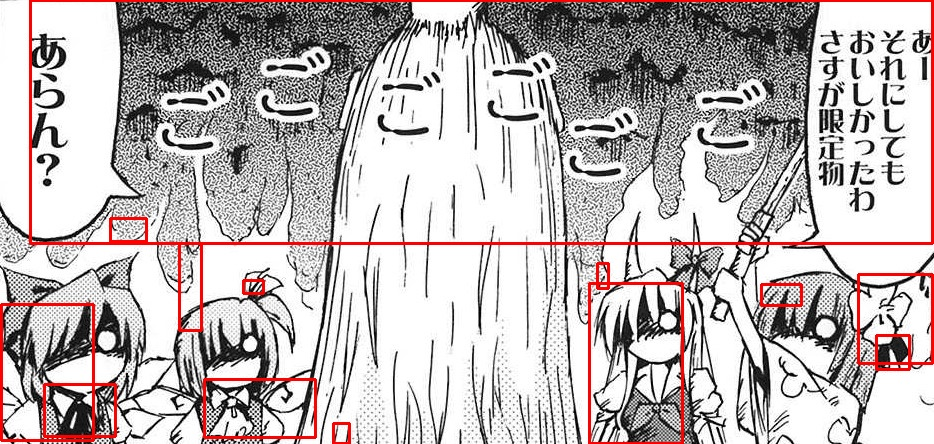
\includegraphics[width=0.7\columnwidth]{images/similar-obj-3.jpg}
        \label{Fig:similar:3}
    }
    \caption{ตัวอย่างผลลัพธ์จากการตรวจหาข้อความบนภาพมังงะด้วยวิธีต้นฉบับ~\cite{5540041} แสดงให้เห็น False Positive จำนวนมาก (ก) นักวาด: Shinoasa (ข) นักวาด: Kousei (Public Planet)}
    \label{Fig:similar}
\end{figure}

ความแตกต่างของวิธีต้นฉบับและวิธีการใหม่ของเรานั้นถูกแสดงให้เห็นในภาพ~\ref{Fig:text_detection_method} อย่างที่เห็นในภาพ~\ref{Fig:text_detection_method:manga}  เราได้เพิ่มขั้นตอนการคัดแยกตัวอักษรเข้ามา โดยวิธีการใหม่จะคัดแยกอักษรออกจากวัตถุอื่น ๆ ที่ไม่มีความเกี่ยวข้องก่อนที่จะจับกลุ่มตัวอักษรเข้าเป็นประโยค ขั้นตอนการคัดแยกนี้ใช้ความสามารถของ SVM Classification เพื่อช่วยลด False Positive ของผลลัพธ์การค้นหาวัตถุที่คล้ายตัวอักษรจากขั้นตอนก่อนหน้า

\begin{figure}[!h]
    \centering
    \subfigure[]{
        \label{Fig:text_detection_method:natural_scene}
        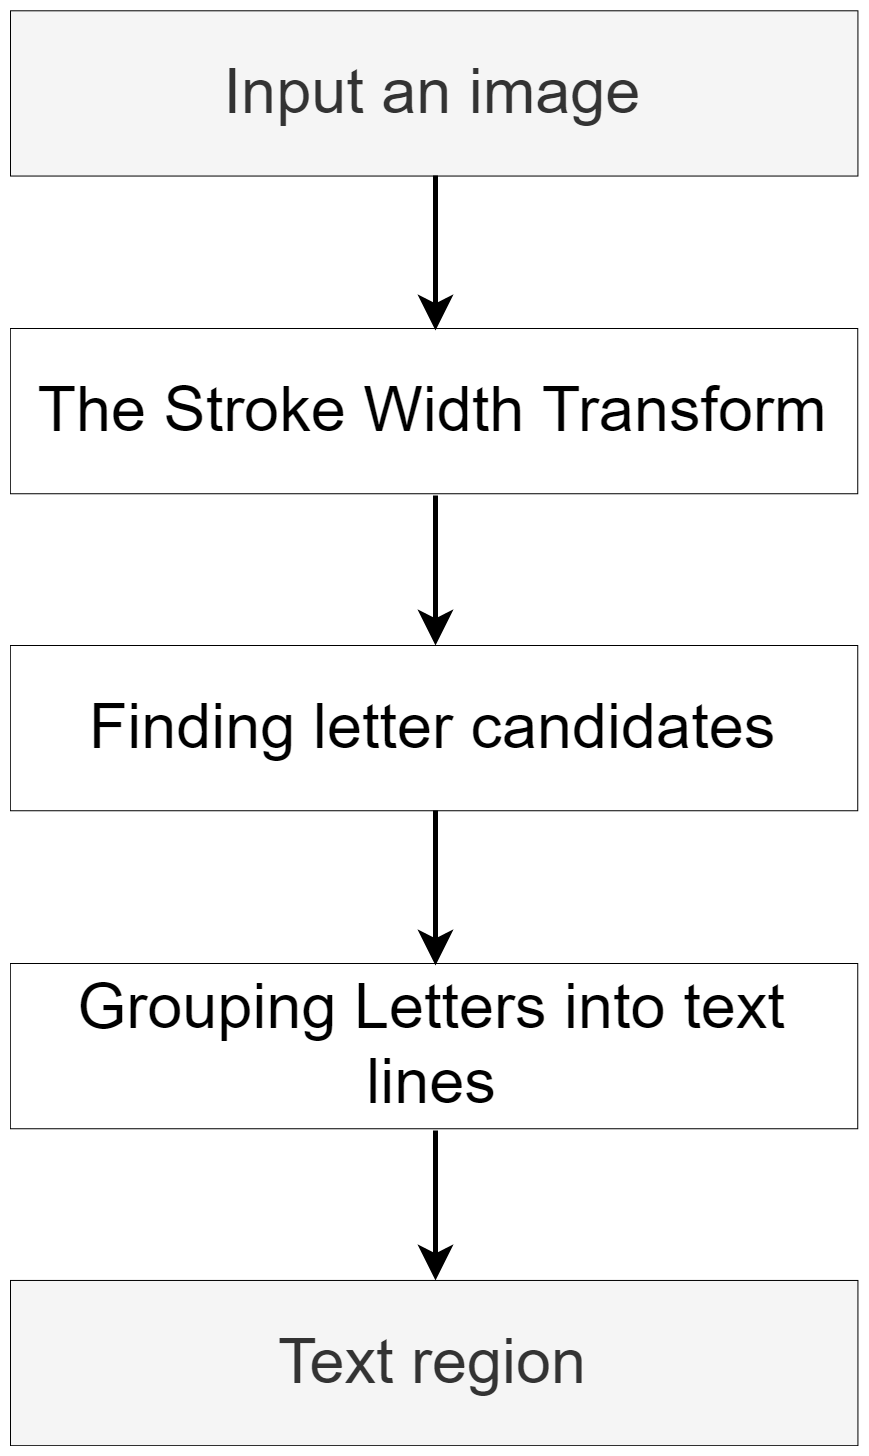
\includegraphics[width=0.3\columnwidth]{detect-text-in-natural-scene.png}  
    }
    \subfigure[]{
        \label{Fig:text_detection_method:manga}
        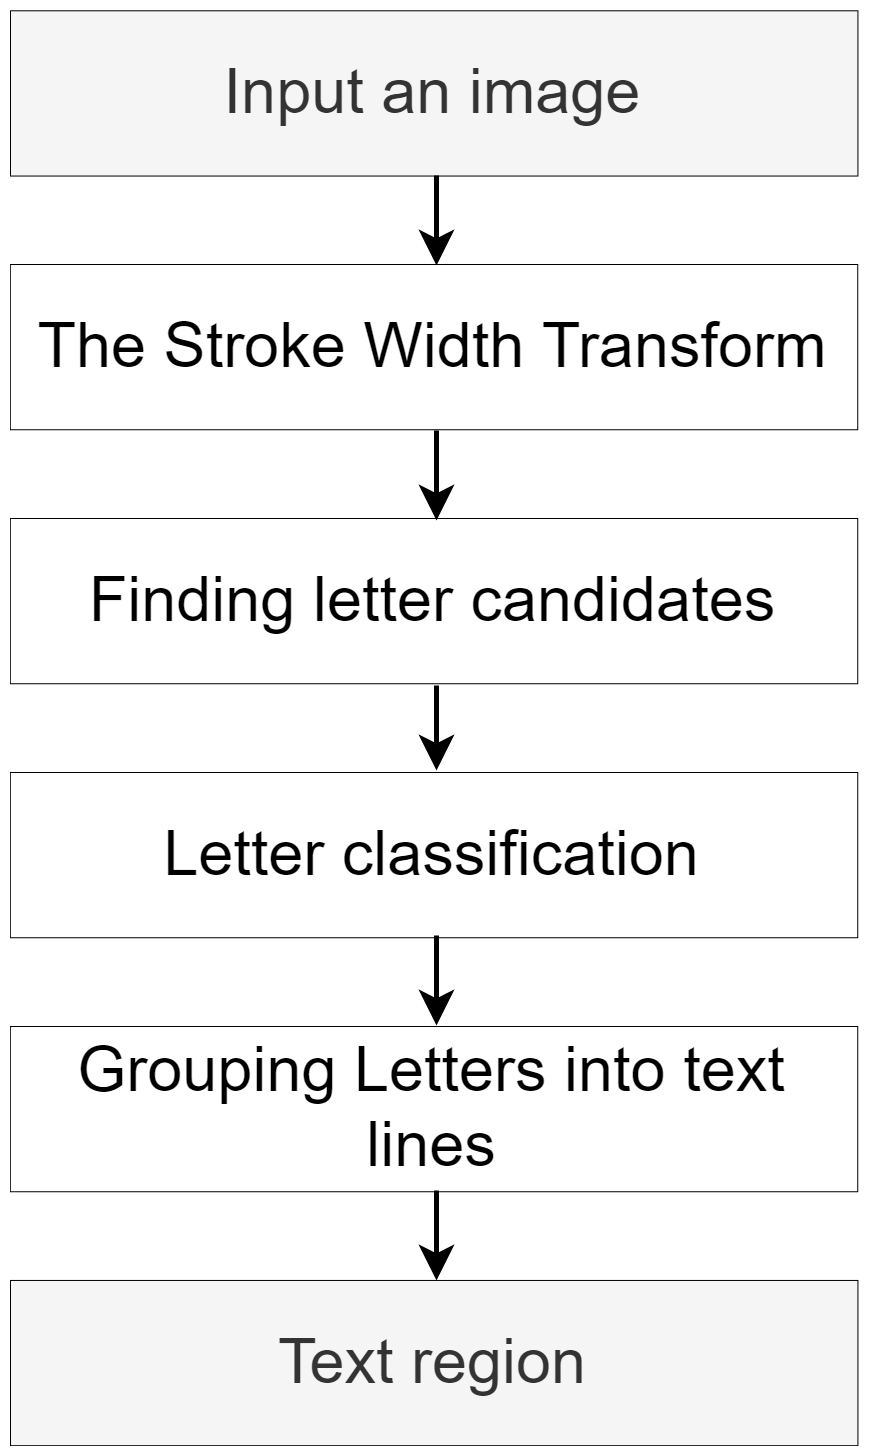
\includegraphics[width=0.3\columnwidth]{our-purposed-method.png}
    }
    \caption{แผนผังการทำงานของ (ก) วิธีการดั้งเดิม~\cite{5540041} และ (ข) วิธีการใหม่ของเรา}
    \label{Fig:text_detection_method}
\end{figure}

\subsection{The Stroke Width Transform}
ในขั้นตอนนี้ใช้วิธีการเดียวกับงานวิจัย~\cite{5540041} ที่กล่าวไปในบทที่~\ref{chapter:related-theory} โดยเรานำ SWT มาดำเนินการบนภาพมังงะเพื่อให้อยู่รูปแบบตัวดำเนินการ SWT โดยข้อมูล Output ของขั้นตอนนี้คือเมทริกซ์ขนาดเท่ากับภาพ Input ซึ่ง Output นี้จะถูกใช้ในขั้นตอนต่อไป

\subsection{ค้นหาวัตถุที่ใกล้เคียงอักษร}
ในมังงะนั้นข้อความหรืออักษรทั้งหลายมีขนาดที่หลากหลายและแตกต่างไปจากภาพถ่าย เราจึงต้องนำกฎเกณฑ์ที่ใช้ในการคัดกรองวัตถุกับตัวอักษรบนภาพถ่ายมากระทำการดัดแปลงให้เหมาะกับสภาพลักษณะเฉพาะของอักษรในมังงะ โดยกฎดังกล่าวถูกดังแปลงให้อยู่ในรูปแบบสมการ~\ref{eq:new-condition}

\begin{equation}
    \begin{split}
        f(d, h, w, \tilde{s}) =
        \begin{cases}
            1, &\text{if } 1 < \frac{d}{\tilde{s}} < 15 \text{ and } \tilde{s} \leq 80 \text{ and } \\ & 5 < h, w < 50 \\
            0, &otherwise,
        \end{cases}
    \end{split}
\label{eq:new-condition}
\end{equation}

โดยตัวแปรใหม่ที่ถูกเพิ่มเข้ามาคือ $w$ ซึ่งคือ ค่าความกว้างของวัตถุนั้น ๆ

เมื่อเรากำจัดวัตถุที่ไม่มีลักษระคล้ายคลึงอักษรออกไปแล้ว เราจะได้กลุ่มของวัตถุที่มีลักษณะใกล้เคียงอักษร อย่างที่แสดงในภาพ~\ref{Fig:sliced-window-testing} โดยในขั้นตอนนี้ของวิธีการ SWT ต้นฉบับไม่สามารถรวบรวมวัตถุที่คล้ายคลึงอักษรได้ครบถ้วนเพียงพอตามที่แสดงให้เห็นในภาพ~\ref{Fig:sliced-window-testing:conventional} แต่กฎใหม่ของเราที่ถูกปรับปรุงแล้วนั้นสามารถรวบรวมวัตถุที่คล้ายอักษรได้ครอบคลุมมากขึ้น อย่างไรก็ดีกฎเกณฑ์ใหม่นั้นสร้าง False Positive ที่มากขึ้นตาม ซึ่งมากกว่าผลลัพธ์จากกฏเกณฑ์ดั้งเดิมของ SWT ต้นฉบับ อย่างไรก็ดีปัญหาดังกล่าวจะถูกแก้ไขด้วยขั้นตอนคัดแยกอักษรด้วย SVM ต่อไป ซึ่ง SVM จะทำหน้าที่กำจัด False Positive ออกไป

\begin{figure}[!t]
    \centering
    \subfigure[]{
        \label{Fig:sliced-window-testing:conventional}
        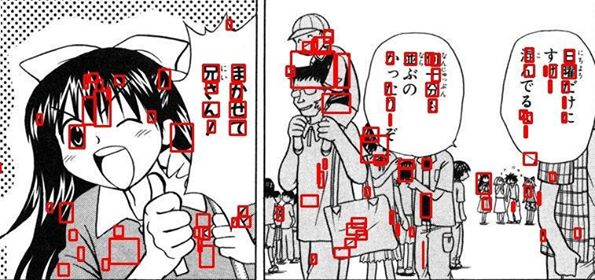
\includegraphics[width=0.95\columnwidth]{conventional-patch.jpg}  
    }
    \subfigure[]{
        \label{Fig:sliced-window-testing:proposed}
        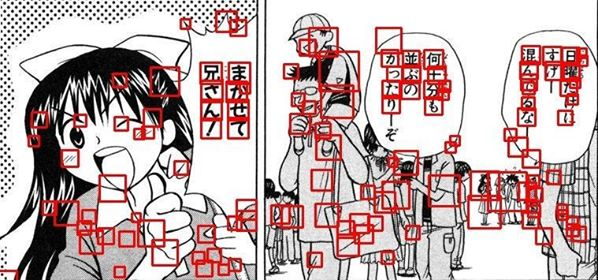
\includegraphics[width=0.95\columnwidth]{proposed-patch.jpg}
    }
    \caption{ตัวอย่างแสดงการเปรียบเทียบผลลัพธ์ระหว่างขอบเขตตัวอักษรที่ตรวจพบระหว่างการใช้กฏเกณฑ์เก่าของ SWT ต้นฉบับ (ก) และกฏเกณฑ์ใหม่ในวิธีของเรา (ข) ข้อมูลภาพถูกนำมาจากเรื่อง Arisa \copyright Yagami Ken}
    \label{Fig:sliced-window-testing}
\end{figure}

\subsection{คัดแยกอักษรด้วย SVM}

ในขั้นตอนนี้เราสร้างภาพขนาดเล็ก (Patch) จากภาพมังงะ Input โดยพึ่งพาตำแหน่งและขนาดของวัตถุที่คล้ายคลึงอักษรจากขั้นตอนก่อนหน้าในการสร้างขอบเขตของภาพขนาดเล็กนั้น ๆ โดยภาพขนาดเล็กเหล่านี้จะถูกคัดแยกเป็นกลุ่มที่เป็นอักษรและกลุ่มที่ไม่ใช่ตัวอักษรด้วย SVM ซึ่งจะช่วยลด False Positive ให้ต่ำลงทำให้ได้ผลลัพธ์การตรวจหาข้อความที่แม่นยำมากขึ้น

เราได้นำ SVM มาดำเนินการในขั้นตอนนี้โดย SVM คือ เทคนิค Supervised Learning แบบหนึ่งซึ่งมักถูกใช้ในงานด้านคัดแยก (Classification) และ สมการถดถอยต่อเนื่อง (Regression)~\cite{Suykens1999} สำหรับชุดข้อมูลสำหรับเทรนโมเดลของ SVM ในขั้นตอนนี้จะถูกสร้างจากภาพขนาดเล็ก หรือ Patch โดยแบ่งออกเป็น ภาพที่เป็นอักษร (Positive) และ ภาพที่ไม่ใช่อักษร (Negative) อย่างทีแสดงในภาพ~\ref{Fig:sliced_window} ภาพขนาดเล็กสำหรับเทรนนิ่งและทดสอบเหล่านี้สร้างจาก Manga109 สำหรับภาพ Positive และ Negative ที่สร้างขึ้นมาจะถูกนำไปสกัดลักษณะเด่นหรือ Feature ด้วย Histogram of Oriented Gradients หรือ HOG~\cite{Freeman} ซึ่งเป็นเทคนิคการสกัดข้อมูลเชิงรูปร่างของวัตถุในภาพด้วยการพึ่งพาการกระจายตัวของทิศทางโทนสี โดยลักษณะเด่นที่ถูกสกัดมาสำหรับใช้งานในงานวิจัยนี้นั้นเป็นข้อมูลรูปแบบเวกเตอร์ 2,916-dimension

เช่นเดียวกับข้อมูลสำหรับเทรน ภาพขนาดเล็กของวัตถุที่คล้ายคลึงอักษรจากขั้นตอนก่อนหน้าจะถูก HOG สกัดลักษณะเด่นออกมาแล้วจึงนำไปให้ SVM ดำเนินการคัดแยกภาพที่เป็นอักษรและไม่ใช่อักษรออกจากกัน หลังจากเสร็จสิ้นกระบวนการ ส่วนภาพที่เป็นอักษรจะถูกนำไปใช้ในการจัดกลุ่มอักษรให้เกิดเป็นข้อความในขั้นตอนต่อไป

\begin{figure}[!h]
    \centering
    \subfigure[]{
        \label{Fig:sliced_window:positive}
        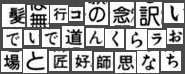
\includegraphics[width=0.45\columnwidth]{ccp-text.jpg}  
    }
    \subfigure[]{
        \label{Fig:sliced_window:negative}
        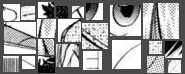
\includegraphics[width=0.45\columnwidth]{ccp-non-text.jpg}  
    }
    \caption{ตัวอย่างของ Patch: (ก) ภาพ Positive Patches and (ข) ภาพ Negative Patches}
    \label{Fig:sliced_window}
\end{figure}

\subsection{จัดกลุ่มอักษรเป็นข้อความ}

ในวิธีการต้นฉบับ~\cite{5540041} ขั้นตอนจัดกลุ่มวัตถุที่คล้ายคลึงอักษรเข้าด้วยกันเป็นประโยคหรือบรรทัดของข้อความได้ใช้หลักการเปรียบเทียบความคล้ายคลึงลักษณะต่าง ๆ ของตัวอักษร ประกอบไปด้วย ของความสูง ขนาดเส้น ทิศทาง และ ระยะห่าง โดยวัตถุที่ไม่ถูกจับคู่จะถูกกำจัดทิ้งไป กระบวนการนี้ใช้สมมติฐานว่าประโยคหรือข้อความมักเกิดจากการรวมตัวกันของอักษรมากกว่าหนึ่งตัวและจัดเรียงอยู่ในทิศทางเดียวกันกับตัวอักษรอื่น ๆ ที่ขนาดใกล้เคียงกันตามที่ได้กล่าวไปใน~\ref{chapter:related-theory} ขั้นตอนนี้ช่วยกำจัดข้อมูลรบกวนอื่น ๆ เช่น วัตถุที่ไม่ใช่อักษรที่กระจายอยู่ในภาพ แต่อย่างไรก็ดี วิธีการของเรานั้นได้กำจัดข้อมูลรบกวนเหล่านี้ออกไปแล้วในขั้นตอนการคัดแยกอักษรด้วย SVM ดังนั้นเราจึงใช้เพียงระยะห่างระหว่างอักษรเป็นปัจจัยในการจับกลุ่มอักษร

วิธีการจัดกลุ่มอักษรของเรานั้นจะใช้อักษรที่ถูกคัดแยกด้วย SVM แล้วมาจัดกลุ่มเป็นประโยคโดยการจัดกลุ่มแต่ละอักษรที่อยู่ห่างกันไม่เกิน 1.5 เท่าของตัวอักษรที่แคบที่สุดของคู่อักษรที่ใช้เปรียบเทียบ หากตัวอักษรใดที่ห่างจากกันเกินกว่าค่าที่กำหนดจะถือว่าเป็นอักษรของคนละประโยคซึ่งจะไม่ถูกจับกลุ่มเข้ามา โดยตัวอย่างในภาพ~\ref{Fig:grouping} แสดงถึงตัวอย่างขั้นตอนการจับกลุ่มด้วยระยะห่าง นอกจากนี้หลังจากการจัดกลุ่มแต่ละประโยคด้วยระยะห่างเสร็จสิ้นแล้ว กลุ่มอักษรเหล่านี้ถูกนำมาพิจารณาขนาดด้วยเช่นกัน โดยแต่ละกลุ่มของอักษรหรือแต่ละข้อความต้องมีพื้นที่ (ความกว้าง $\times$ ความสูง) เกินกว่า 2,550px อ้างอิงจากการทดลองกับชุดข้อมูลของเรา สุดท้ายเราจะได้กลุ่มของอักษรหรือประโยคข้อความจากภาพในมังงะออกมา

\begin{figure}[!t]
    \centering
    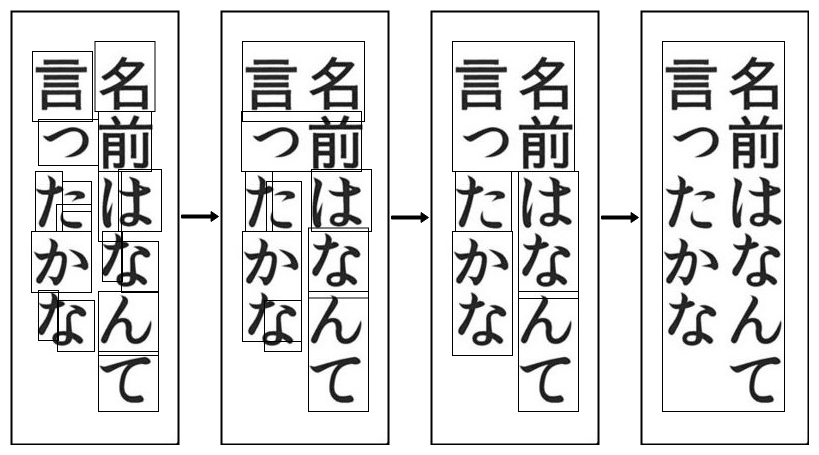
\includegraphics[width=0.6\columnwidth]{grouping.png}
    \caption{ตัวอย่างแสดงการจับกลุ่มของตัวอักษร}
    \label{Fig:grouping}
\end{figure}

\section{ชุดข้อมูลสำหรับการเทรนโมเดล SVM}

เราได้นำภาพจากชุดข้อมูลภาพมังงะขนาดใหญ่ Manga109~\cite{Matsui2017} ประกอบไปด้วยภาพมังงะพร้อมข้อมูลประกอบ หรือ Annotation ของมังงะ 109 เรื่อง จัดทำโดยห้องทดลอง Aizawa Yamasaki แห่งมหาวิทยาลัยโตเกียว มังงะทั้งหมดในชุดข้อมูลนี้ถูกวาดโดยนักวาดมังงะมืออาชีพชาวญี่ปุ่นและถูกจัดจำหน่ายในช่วงปี 1970 ถึงปี 2010 แต่ละหน้าของมังงะถูกระบุตำแหน่งของข้อความในภาพซึ่งข้อมูลดังกล่าวนี้เหมาะแก่การใช้เทรนโมเดลและทดสอบวิธีการของเรา

\section{การทดลอง}

เราดำเนินการทดลองในรูปแบบเดียวกับงานวิจัยของ Aramaki et al.~\cite{7532890} ซึ่งจะทำให้เราสามารถเปรียบเทียบผลการทดลองประสิทธิภาพวิธีการของเรากับงานวิจัยอื่น ๆ ที่เกี่ยวข้องกับการตรวจหาข้อความในภาพมังงะซึ่งเคยถูกทดสอบมาก่อนหน้าแล้วได้ เราได้เลือกภาพมังงะด้วยวิธีการสุ่มเลือก 100 หน้าสำหรับการเทรน และอีก 100 หน้าสำหรับทดสอบประสิทธิภาพ โดยภาพมังงะทั้งหมดนี้ถูกสุ่มเลือกจากมังงะ 6 เรื่อง ได้แก่ \textit{Aosugiru Haru, Arisa 2, Bakuretsu Kung Fu Girl, Dollgun, Love Hina,} และ \textit{Uchiha Akatsuki EvaLady}

เนื่องจากวิธีการของเราใช้ SVM ซึ่งต้องสร้างโมเดลสำหรับใช้งานคัดแยกภาพระหว่างภาพขนาดเล็ก (Patch) ระหว่างกลุ่มที่เป็นอักษรและไม่ใช่อักษรตามที่แสดงไปในภาพ~\ref{Fig:sliced_window} เราจึงได้สร้างชุดข้อมูลประกอบด้วยภาพอักษร 5,201 ภาพ และ ภาพขนาดเล็กอื่น ๆ ของวัตถุที่ไม่ใช่อักษรอีก 5,201 ภาพ กล่าวคือแบ่งเป็นข้อมูล Positive และ Negative ส่วนละ 50\% เท่า ๆ กัน โดยภาพเหล่านี้สร้างจากภาพสำหรับการเทรนที่ได้ถูกกล่าวไปในย่อหน้าก่อนหน้า โดยใช้ขั้นตอน \textit{ค้นหาวัตถุที่ใกล้เคียงอักษร} ของเราในการค้นหาตำแหน่งและขอบเขตของวัตถุที่คล้ายคลึงอักษรและนำตำแหน่งเหล่านั้นสร้างภาพขนาดเล็กเหล่านี้ออกมา

สำหรับ SVM เราใช้ Radial Basis Function Kernel โดย Hyperparameter ที่ร่วมใช้งานประกอบไปด้วย $C$ และ $\gamma$ เราใช้ Grid Search บนเครื่องคอมพิวเตอร์ \textit{Google Cloud Compute Engine n1-highcpu-8} ในการค้นหาค่า Hyperparameter ที่ดีที่สุด ในช่วง $2^{-10}$ ถึง $2^{10}$ โดยได้ค่า $C$ และ $\gamma$ ที่ดีที่สุดที่ $2^5$ และ $2^{-6.75}$ ตามลำดับ โมเดลที่ถูกปรับปรุงให้เหมาะสม (Optimized) แล้วนี้จะถูกนำไปใช้ในขั้นตอนคัดแยกอักษรด้วย SVM

การประเมินวิธีการของเราที่ถูกพัฒนาขึ้นใหม่นั้นได้ใช้รูปแบบการประเมินเดียวกับที่ใช้ใน ICDAR 2013 Robust Reading Competition~\cite{6628859} โดยถ้าอัตราส่วนระหว่างพื้นที่ Overlapped ต่อ พื้นที่ Ground-truth นั้นมากกว่าค่า $t_p$  และอัตราส่วนระหว่างพื้นที่ Overlapped ต่อ พื้นที่ Detected Region มากกว่า $t_r$ ให้ถือว่า พื้นที่ขอบเขตอักษรที่ถูกตรวจพบจากวิธีการของเรานั้นถูกต้อง โดย $t_p$ และ $t_r$ นั้นมีค่าเท่ากับ 0.5 อ้างอิงค่าดังกล่าวตามงานวิจัยของ Aramaki et al.~\cite{7532890} สำหรับ Precision และ Recall เราได้คำนวณตามสมการดังต่อไปนี้~\ref{eq:precision}, ~\ref{eq:recall} ตามลำดับ

\begin{eqnarray}
    P&=& \frac{\text{\#Correctly Detected Rectangles}}{\text{\#Detected Rectangles}}\label{eq:precision}\\
    R&=& \frac{\text{\#Correctly Detected Rectangles}}{\text{\#Rectangles of the Ground-truth}}\label{eq:recall}
\end{eqnarray}

สำหรับ F-Measure เราคำนวนด้วยสมการดังนี้~\ref{eq:fmeasure}

\begin{equation}
    F = 2\cdot\frac{P \cdot R}{P+R}
    \label{eq:fmeasure}
\end{equation}

เราได้เปรียบเทียบผลการทดลองของวิธีการใหม่ของเราร่วมกับวิธีการต้นฉบับ~\cite{Suykens1999} ซึ่งถูกใช้กับภาพถ่าย นอกจากนี้ยังเปรียบเทียบกับงานวิจัยการตรวจหาข้อความอื่น ๆ ด้วย ดังนี้ Basic Grouping+ImageNet Classification Model (BG+ImN)~\cite{7532890}, Basic Grouping+Illustration2Vec Model (BG+I2V)~\cite{7532890}, Scene Text Detection (STD)~\cite{6628665}, Speech Balloon Detection (SBD)~\cite{6761596}, และ Text Line Detection (TLD)~\cite{rigaud:hal-00841492} วิธีข้างต้นที่กล่าวถึงมีเทคนิคในการตรวจหาข้อความที่หลากหลายแตกต่างกัน เช่น การยึดหลักสมมติฐานพื้นฐาน (ทิศทางของข้อความ, รูปแบบการจัดวาง, ลักษณะของกล่องคำพูด) และ Convolutional nueral network 

สำหรับ BG+ImN, BG+I2V, STD, SBD, และ TLD นั้นเราได้นำผลลัพทธ์การทดลองจากงานวิจัยของ Aramaki et al.~\cite{7532890} มาใช้ในการเปรียบของเราโดยตรง ซึ่งการเปรียบเทียบโดยตรงนี้สามารถทำได้เนื่องจากเราได้ดำเนินการทดลองในสภาพแบบเดียวกับงานวิจัยดังกล่าว โดยผลลัพธ์การเปรียบเทียบและตัวอย่างขอบเขตข้อความที่วิธีการของเรานั้นสามารถตรวจพบถูกแสดงให้บทที่~\ref{chapter:result}